\documentclass{beamer}

% xcolor and define colors -------------------------
\usepackage{xcolor}

% https://www.viget.com/articles/color-contrast/
\definecolor{purple}{HTML}{5601A4}
\definecolor{navy}{HTML}{0D3D56}
\definecolor{ruby}{HTML}{9a2515}
\definecolor{alice}{HTML}{107895}
\definecolor{daisy}{HTML}{EBC944}
\definecolor{coral}{HTML}{F26D21}
\definecolor{kelly}{HTML}{829356}
\definecolor{cranberry}{HTML}{E64173}
\definecolor{jet}{HTML}{131516}
\definecolor{asher}{HTML}{555F61}
\definecolor{slate}{HTML}{314F4F}

% Mixtape Sessions
\definecolor{picton-blue}{HTML}{00b7ff}
\definecolor{violet-red}{HTML}{ff3881}
\definecolor{sun}{HTML}{ffaf18}
\definecolor{electric-violet}{HTML}{871EFF}

\newcommand\pictonBlue[1]{{\color{picton-blue}#1}}
\newcommand\sun[1]{{\color{sun}#1}}
\newcommand\electricViolet[1]{{\color{electric-violet}#1}}
\newcommand\violetRed[1]{{\color{violet-red}#1}}

\newcommand\bgPictonBlue[1]{{\colorbox{picton-blue!20!white}{#1}}}
\newcommand\bgSun[1]{{\colorbox{sun!20!white}{#1}}}
\newcommand\bgElectricViolet[1]{{\colorbox{electric-violet!20!white}{#1}}}
\newcommand\bgVioletRed[1]{{\colorbox{violet-red!20!white}{#1}}}

\def\code#1{\texttt{#1}}

% Main theme colors
\definecolor{accent}{HTML}{00b7ff}
\definecolor{accent2}{HTML}{871EFF}
\definecolor{gray100}{HTML}{f3f4f6}
\definecolor{gray800}{HTML}{1F292D}


% Beamer Options -------------------------------------

% Background
\setbeamercolor{background canvas}{bg = white}

% Change text margins
\setbeamersize{text margin left = 15pt, text margin right = 15pt} 

% \alert
\setbeamercolor{alerted text}{fg = accent2}

% Frame title
\setbeamercolor{frametitle}{bg = white, fg = jet}
\setbeamercolor{framesubtitle}{bg = white, fg = accent}
\setbeamerfont{framesubtitle}{size = \small, shape = \itshape}

% Block
\setbeamercolor{block title}{fg = white, bg = accent2}
\setbeamercolor{block body}{fg = gray800, bg = gray100}

% Title page
\setbeamercolor{title}{fg = gray800}
\setbeamercolor{subtitle}{fg = accent}

%% Custom \maketitle and \titlepage
\setbeamertemplate{title page}
{
    %\begin{centering}
        \vspace{20mm}
        {\Large \usebeamerfont{title}\usebeamercolor[fg]{title}\inserttitle}\\
        {\large \itshape \usebeamerfont{subtitle}\usebeamercolor[fg]{subtitle}\insertsubtitle}\\ \vspace{10mm}
        {\insertauthor}\\
        {\color{asher}\small{\insertdate}}\\
    %\end{centering}
}

% Table of Contents
\setbeamercolor{section in toc}{fg = accent!70!jet}
\setbeamercolor{subsection in toc}{fg = jet}

% Button 
\setbeamercolor{button}{bg = accent}

% Remove navigation symbols
\setbeamertemplate{navigation symbols}{}

% Table and Figure captions
\setbeamercolor{caption}{fg=jet!70!white}
\setbeamercolor{caption name}{fg=jet}
\setbeamerfont{caption name}{shape = \itshape}

% Bullet points

%% Fix spacing between items
\let\olditemize=\itemize 
\let\endolditemize=\enditemize 
\renewenvironment{itemize}{\vspace{0.25em}\olditemize \itemsep0.25em}{\endolditemize}

%% Fix left-margins
\settowidth{\leftmargini}{\usebeamertemplate{itemize item}}
\addtolength{\leftmargini}{\labelsep}

%% enumerate item color
\setbeamercolor{enumerate item}{fg = accent}
\setbeamerfont{enumerate item}{size = \small}
\setbeamertemplate{enumerate item}{\insertenumlabel.}

%% itemize
\setbeamercolor{itemize item}{fg = accent!70!white}
\setbeamerfont{itemize item}{size = \small}
\setbeamertemplate{itemize item}[circle]

%% right arrow for subitems
\setbeamercolor{itemize subitem}{fg = accent!60!white}
\setbeamerfont{itemize subitem}{size = \small}
\setbeamertemplate{itemize subitem}{$\rightarrow$}

\setbeamertemplate{itemize subsubitem}[square]
\setbeamercolor{itemize subsubitem}{fg = jet}
\setbeamerfont{itemize subsubitem}{size = \small}








% Links ----------------------------------------------

\usepackage{hyperref}
\hypersetup{
  colorlinks = true,
  linkcolor = accent2,
  filecolor = accent2,
  urlcolor = accent2,
  citecolor = accent2,
}


% Line spacing --------------------------------------
\usepackage{setspace}
\setstretch{1.35}


% \begin{columns} -----------------------------------
\usepackage{multicol}


% Fonts ---------------------------------------------
% Beamer Option to use custom fonts
\usefonttheme{professionalfonts}

% \usepackage[utopia, smallerops, varg]{newtxmath}
% \usepackage{utopia}
\usepackage[sfdefault,light]{roboto}

% Small adjustments to text kerning
\usepackage{microtype}



% Remove annoying over-full box warnings -----------
\vfuzz2pt 
\hfuzz2pt


% Table of Contents with Sections
\setbeamerfont{myTOC}{series=\bfseries, size=\Large}
\AtBeginSection[]{
        \frame{
            \frametitle{Roadmap}
            \tableofcontents[current]   
        }
    }


% Tables -------------------------------------------
% Tables too big
% \begin{adjustbox}{width = 1.2\textwidth, center}
\usepackage{adjustbox}
\usepackage{array}
\usepackage{threeparttable, booktabs, adjustbox}
    
% Fix \input with tables
% \input fails when \\ is at end of external .tex file
\makeatletter
\let\input\@@input
\makeatother

% Tables too narrow
% \begin{tabularx}{\linewidth}{cols}
% col-types: X - center, L - left, R -right
% Relative scale: >{\hsize=.8\hsize}X/L/R
\usepackage{tabularx}
\newcolumntype{L}{>{\raggedright\arraybackslash}X}
\newcolumntype{R}{>{\raggedleft\arraybackslash}X}
\newcolumntype{C}{>{\centering\arraybackslash}X}

% Figures

% \imageframe{img_name} -----------------------------
% from https://github.com/mattjetwell/cousteau
\newcommand{\imageframe}[1]{%
    \begin{frame}[plain]
        \begin{tikzpicture}[remember picture, overlay]
            \node[at = (current page.center), xshift = 0cm] (cover) {%
                \includegraphics[keepaspectratio, width=\paperwidth, height=\paperheight]{#1}
            };
        \end{tikzpicture}
    \end{frame}%
}

% subfigures
\usepackage{subfigure}


% Highlight slide -----------------------------------
% \begin{transitionframe} Text \end{transitionframe}
% from paulgp's beamer tips
\newenvironment{transitionframe}{
    \setbeamercolor{background canvas}{bg=accent!40!black}
    \begin{frame}\color{accent!10!white}\LARGE\centering
}{
    \end{frame}
}


% Table Highlighting --------------------------------
% Create top-left and bottom-right markets in tabular cells with a unique matching id and these commands will outline those cells
\usepackage[beamer,customcolors]{hf-tikz}
\usetikzlibrary{calc}
\usetikzlibrary{fit,shapes.misc}

% To set the hypothesis highlighting boxes red.
\newcommand\marktopleft[1]{%
    \tikz[overlay,remember picture] 
        \node (marker-#1-a) at (0,1.5ex) {};%
}
\newcommand\markbottomright[1]{%
    \tikz[overlay,remember picture] 
        \node (marker-#1-b) at (0,0) {};%
    \tikz[accent!80!jet, ultra thick, overlay, remember picture, inner sep=4pt]
        \node[draw, rectangle, fit=(marker-#1-a.center) (marker-#1-b.center)] {};%
}


% DAGS ----------------------------------------------
\usepackage{tikz}
\usetikzlibrary{shapes,decorations,arrows,calc,arrows.meta,fit,positioning}
% Tikz settings optimized for causal graphs.
\tikzset{
    -Latex,auto,node distance =1 cm and 1 cm,semithick,
    state/.style ={ellipse, draw, minimum width = 0.7 cm},
    point/.style = {circle, draw, inner sep=0.04cm,fill,node contents={}},
    bidirected/.style={Latex-Latex,dashed},
    el/.style = {inner sep=2pt, align=left, sloped}
}


% Beamer tricks -------------------------------------
% Make \pause work in align environments
\makeatletter
\renewrobustcmd{\beamer@@pause}[1][]{%
  \unless\ifmeasuring@%
  \ifblank{#1}%
    {\stepcounter{beamerpauses}}%
    {\setcounter{beamerpauses}{#1}}%
  \onslide<\value{beamerpauses}->\relax%
  \fi%
}
\makeatother




\begin{document}

\imageframe{./lecture_includes/cover_intro.png}

\section{Introductions}

\subsection{Who Am I?}
\subsection{Who Am I?}
\begin{frame}{Who Am I?}

Groos Family Assistant Professor of Economics, Brown University\pause

A big fan of instrumental variable (IV) methods\pause
\begin{itemize}
  \item Lottery- and non-lottery IVs in studies of educational quality \\ {\scriptsize \textcolor{red!75!green!50!blue!25!gray}{(Angrist et al. 2016, 2017, 2021, 2022; Abdulkadiro\u{g}lu et al. 2016)}}
  \item Quasi-experimental evaluations of healthcare quality \\ {\scriptsize \textcolor{red!75!green!50!blue!25!gray}{(Hull 2020; Abaluck et al. 2021, 2022)}}
  \item IV-based analyses of discrimination and bias \\ {\scriptsize \textcolor{red!75!green!50!blue!25!gray}{(Arnold et al. 2020, 2021, 2022; Hull 2021; Bohren et al. 2022)}}
  \item Shift-share instruments and related designs \\ {\scriptsize \textcolor{red!75!green!50!blue!25!gray}{(Borusyak et al. 2022; Borusyak and Hull 2021, 2022; Goldsmith-Pinkham et al. 2022)}}
\end{itemize}\pause

A constant student of IV (and econometrics more generally)

\end{frame}

\subsection{What is This Course?}
\begin{frame}{What is This Course?}

A one-day intensive on IV, with focus on recent practical advances \pause

\begin{itemize}
  \item Far from comprehensive; stay tuned for more ``mixtape tracks'' that take deeper dives on particular topics (judge IV, etc)
  \item Emphasis on \emph{practical}: IV is meant to be used, not just studied!
\end{itemize}\pause\medskip

Four one-hour lectures: from IV basics to recent topics\pause

\begin{itemize}
  \item Please ask questions in the Discord chat!
  \item I will try to stick to the schedule but may improvise slightly
\end{itemize}\pause\medskip

Two 75-minute coding labs, applying what we've learned\pause
\begin{itemize}
  \item I will be live-coding in Stata, but R code will also be available
  \item Goal: demonstrate both methods \& how I think about applying them
\end{itemize}

\end{frame}

\begin{frame}{Schedule}
\includegraphics[scale=0.55]{./lecture_includes/schedule.png}
\end{frame}

\section{Regression Review}

\subsection{Models vs. Estimands vs. Estimators}
\begin{frame}{Models vs. Estimands vs. Estimators}

Three distinct objects (though not always clearly distinguished) \pause\medskip

\begin{itemize}

  \item \bgVioletRed{Parameters} come from models of how observed data are generated
  \begin{itemize}
    \item E.g. a structural supply/demand model or potential outcomes
    \item They set the target for an empirical analysis: what we want to know
  \end{itemize}\pause
  
  \item \bgPictonBlue{Estimands} are functions of the population distribution of observable data
  \begin{itemize}
    \item E.g. a difference in means or ratio of population regression coef's
    \item Make assumptions to link parameters \& estimands (``identification'')
  \end{itemize}\pause
  
  \item \bgSun{Estimators} are functions of the observed data itself (the ``sample'')
  \begin{itemize}
    \item E.g. a difference in sample means or ratio of OLS coefficients 
    \item Since data are random, so are estimators. Each has a distribution
    \item Use knowledge of estimator distributions to make learn about estimands (``inference'') and---hopefully---identified parameters
  \end{itemize}
\end{itemize}
\end{frame}

\begin{frame}{Identification vs. Estimation}


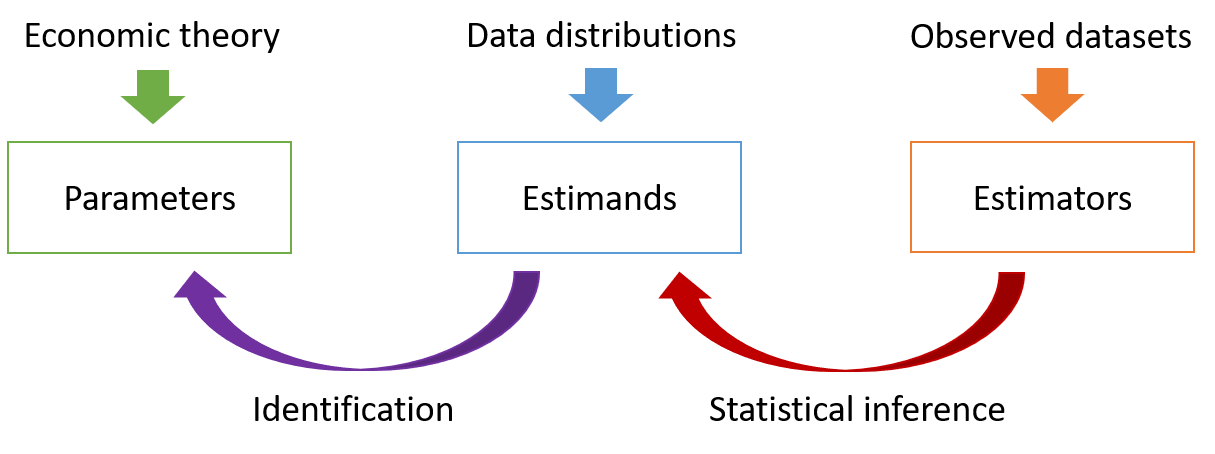
\includegraphics[scale=0.37]{./lecture_includes/BigPicture.png}
\medskip

This course will mostly focus on identification, but we'll cover some IV estimation / inference issues as well
\end{frame}

\subsection{Regression Identification and Endogeneity}
\begin{frame}{Let's Get Concrete}
Human capital theory (e.g. Becker, 1957) tells us that taking one-day IV intensives are likely to boost later-life productivity\pause
\begin{itemize}
  \item Parameter: returns to taking this class $\violetRed{\beta}$ {\small(parameter!!)}, measured in some outcome $Y_i$ (e.g. lifetime top-5 pubs / earnings / twitter followers)
  \item Simple causal/structural model: $Y_i= \alpha + \violetRed{\beta} D_i + \varepsilon_i$, where $D_i \in \{0,1\}$ indicates taking this class
\end{itemize}\pause

We see a sample of $Y_i$, $\violetRed{D_i}$, and some other covariates $W_{1i},\dots,W_{Ki}$
\begin{itemize}
  \item We fire up Stata and \code{reg y d w1-wk, r}. How do we interpret the output?
\end{itemize}

\end{frame}

\begin{frame}{Population Regression}
  The OLS \emph{estimator} $\sun{\widehat{\beta}^{OLS}}$ consistently estimates the regression \emph{estimand} $\pictonBlue{\beta^{OLS}}$ under relatively weak conditions (e.g. \emph{i.i.d.} data)
  \begin{itemize}
  \item Stata tells us $\sun{\widehat{\beta}^{OLS}}$ and what we can infer about $\pictonBlue{\beta^{OLS}}$ from it
  \item It \emph{doesn't} directly tell us about the relationship between $\pictonBlue{\beta^{OLS}}$ and $\violetRed{\beta}$
  \end{itemize}
\end{frame}

\begin{frame}{Population Regression}

The \bgPictonBlue{population regression} of $Y_i$ on $\mathbf{X}_i=[1, \violetRed{D_i},W_{1i},\dots,W_{Ki}]^\prime$ is given by $Y_i=\mathbf{X}_i^\prime \pictonBlue{\beta^{OLS}} + U_i$ where $E[\mathbf{X}_i U_i]=0$\pause
\begin{itemize}
  \item Equivalently, $\pictonBlue{\beta^{OLS}} = E[\mathbf{X}_i\mathbf{X}_i^\prime]^{-1}E[\mathbf{X}_i Y_i]$ and $U_i = Y_i - \mathbf{X}_i^\prime \pictonBlue{\beta^{OLS}} $\smallskip
\item $\pictonBlue{\beta^{OLS}} $ contains regression \emph{coefficients}; $U_i$ is the regression \emph{residual} 
\end{itemize}\medskip\pause


Key point: we can always define $\pictonBlue{\beta^{OLS}} $ for any $Y_i$ and $\mathbf{X}_i$ (assuming no perfect collinearity); this is what Stata estimates
\begin{itemize}
  \item Specifically it computes $\sun{\widehat{\beta}^{OLS}} = (\frac{1}{N}\sum_i\mathbf{X}_i\mathbf{X}_i^\prime)^{-1}(\frac{1}{N}\sum_i\mathbf{X}_iY_i)$ and uses large-sample asymptotics (LLN/CLT) to get a standard error
\end{itemize}

\end{frame}

\begin{frame}{You Can't Always Get What you Want...}
But what if this \emph{estimand} is not what we want? \pause
\begin{itemize}
  \item What if $\pictonBlue{\beta^{OLS}}$ fails to coincide with our economic parameter of interest (e.g. returns to mixtape workshops)?
\end{itemize}
\end{frame}



\begin{frame}{You Can't Always Get What you Want...}

The model parameter in $Y_i=\alpha+ \violetRed{\beta} D_i+\varepsilon_i$ need not coincide with the regression coefficient in $Y_i= \alpha^{OLS} + \pictonBlue{\beta^{OLS}} D_i+U_i$
\begin{itemize}
  \item I.e. we may not have $Cov(D_i,\varepsilon_i)=0$ (always have $Cov(D_i,U_i)=0)$
\end{itemize}\bigskip\pause

Selection bias (a.k.a. omitted variables bias): students with higher latent earnings potential $\varepsilon_i$ are more likely to take this class $D_i$
\begin{itemize}
  \item $Cov(D_i,\varepsilon_i)>0$ means $\pictonBlue{\beta^{OLS}} > \violetRed{\beta}$: overstate the returns-to-mixtape
\end{itemize}\bigskip\pause
\end{frame}

\begin{frame}{Can I just Control My Way Out of This?}

Adding more controls (e.g. demographics) may or may not help
\begin{itemize}
  \item Projecting $\varepsilon_i$ on $X_i$, we get $Y_i=\alpha+ \violetRed{\beta} D_i + \gamma X_i + \tilde\varepsilon_i$, $Cov(X_i,\tilde\varepsilon_i)=0$
  \item Whether or not $Cov(D_i,\tilde\varepsilon_i)=0$ depends on whether $X_i$ sufficiently accounts for the confounding relationship $Cov(D_i,\varepsilon_i)\neq 0$
\end{itemize}
\end{frame}

\begin{frame}{Regression ``Exogeneity''}

\begin{center}
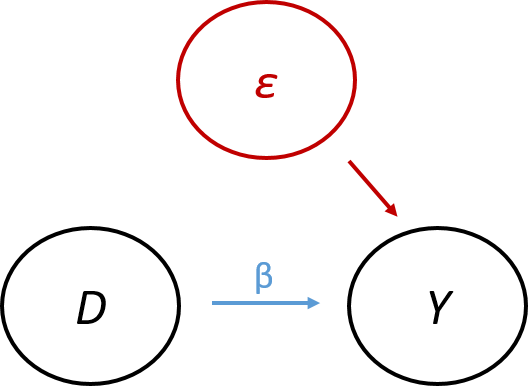
\includegraphics[scale=0.8]{./lecture_includes/dag1.png}
\end{center}

\end{frame}

\begin{frame}{Regression ``Endogeneity''}

\begin{center}
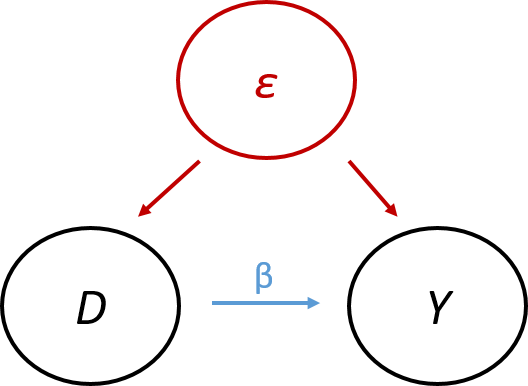
\includegraphics[scale=0.8]{./lecture_includes/dag2.png}
\end{center}

\end{frame}

\begin{frame}{...But Sometimes, You Get What you Need}

Imagine this course was ``oversubscribed,'' and admission was determined by lottery
\begin{itemize}
  \item Among those interested in taking the course, a random sample denoted by $\electricViolet{Z_i} = 1$ was given access
  \item The rest, with $\electricViolet{Z_i} = 0$ not initially given access (maybe got in later)
\end{itemize}\medskip\pause

Intuitively, this external shock $\electricViolet{Z_i}$ should be helpful for identifying $\violetRed{\beta}$
\begin{itemize}
  \item Affects $D_i$, so relevant to the ``treatment'' of interest
  \item Randomly assigned, so unconfounded by selection (unlike $D_i$)
\end{itemize}\medskip\pause

Indeed, this leads us to IV estimands (and estimators)

\end{frame}

\begin{frame}{The IV Solution}

\begin{center}
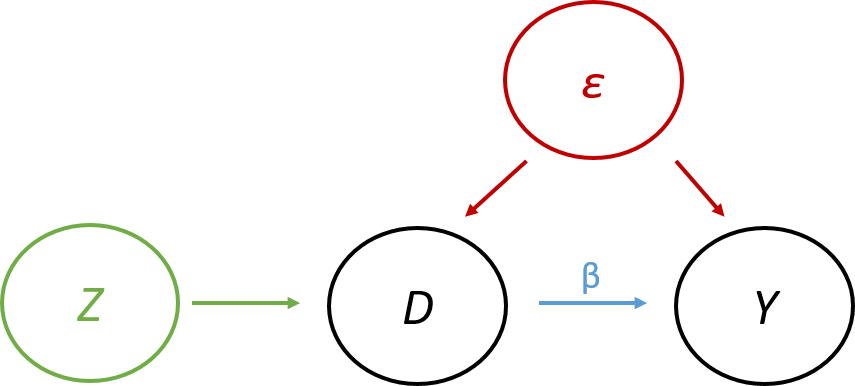
\includegraphics[scale=0.8]{./lecture_includes/dag3.png}
\end{center}

\end{frame}

\section{Intro to IV}

\subsection{Instrument Validity and Relevance}
\begin{frame}{Instrument Validity and Relevance}

Causal/structural model $Y_i=\alpha+ \violetRed{\beta} D_i+\varepsilon_i$ and a candidate IV $Z_i$ 
\begin{itemize}
  \item Single $D_i$ and $Z_i$ and no further controls, for now
\end{itemize}\medskip\pause

Two key assumptions:
\begin{itemize}
  \item Relevance: $Z_i$ and $D_i$ are correlated: $Cov(Z_i,D_i)\neq 0$ 
  \item Validity: $Z_i$ and $\varepsilon_i$ are \emph{un}correlated: $Cov(Z_i,\varepsilon_i)=0$
\end{itemize}\medskip\pause

We then have identification:\vspace{-0.3cm}
\begin{align*}
Cov(Z_i,Y_i) &= Cov(Z_i,\alpha + \violetRed{\beta} D_i+\varepsilon_i)= \violetRed{\beta} Cov(Z_i,D_i)+Cov(Z_i,\varepsilon_i)\\
&= \violetRed{\beta} Cov(Z_i,D_i)\text{, Implying $\violetRed{\beta} = \frac{Cov(Z_i,Y_i)}{Cov(Z_i,D_i)}$}
\end{align*}\pause\vspace{-0.3cm}

$\pictonBlue{\beta^{IV}} = \frac{Cov(Z_i,Y_i)}{Cov(Z_i,D_i)}$ is the (simple) IV \emph{estimand}\pause
\begin{itemize}
\item Compare to the OLS estimand: $\pictonBlue{\beta^{OLS}}=\frac{Cov(D_i,Y_i)}{Var(D_i)}$ 
\end{itemize}

\end{frame}

\begin{frame}{``Reduced Form'' and ``First Stage''}

Note we can write 
\begin{align*}
\pictonBlue{\beta^{IV}} =\frac{Cov(Z_i,Y_i)}{Cov(Z_i,D_i)}=\frac{Cov(Z_i,Y_i)/Var(Z_i)}{Cov(Z_i,D_i)/Var(Z_i)}=\frac{\pictonBlue{\rho^{OLS}}}{\pictonBlue{\pi^{OLS}}}
\end{align*}
where $\pictonBlue{\rho^{OLS}}$ and $\pictonBlue{\pi^{OLS}}$ are two OLS estimands:\pause
\begin{align*}
Y_i &= \kappa^{OLS} + \pictonBlue{\rho^{OLS}} Z_i + V_i \hspace{0.2cm}\text{ ``reduced form''}\\
D_i &= \mu^{OLS} + \pictonBlue{\pi^{OLS}} Z_i + W_i\hspace{0.2cm}\text{ ``first stage''}
\end{align*}\vspace{-0.5cm}\pause

Sometimes we refer to the IV estimand as the ``second stage'':
\begin{align*}
Y_i=\alpha^{IV}+ \pictonBlue{\beta^{IV}} D_i+ U_i
\end{align*}

where now $Cov(Z_i,U_i)=0$. Thus ``IV=RF/FS'' ($\pictonBlue{\beta^{IV}} =\pictonBlue{\rho^{OLS}}/\pictonBlue{\pi^{OLS}}$)

\end{frame}

\subsection{The 2SLS Estimator}
\begin{frame}{The 2SLS Estimator}

  As with OLS, we estimate IV by sample analog:
\begin{align*}
\sun{\widehat\beta^{IV}} = \frac{\widehat{Cov}(Z_i,Y_i)}{\widehat{Cov}(Z_i,D_i)} = \frac{\sun{\widehat\rho^{OLS}}}{\sun{\widehat\pi^{OLS}}}
\end{align*}
where $\widehat{Cov}(X_i,W_i)=\frac{1}{N}\sum_i X_iW_i-\left(\frac{1}{N}\sum_i X_i\right)\left(\frac{1}{N}\sum_i W_i\right)$, $\hat\rho^{OLS}=\widehat{Cov}(Z_i,Y_i)/\widehat{Var}(Z_i)$, and $\hat\pi^{OLS}=\widehat{Cov}(Z_i,D_i)/\widehat{Var}(Z_i)$

\begin{itemize}\pause
\item This is what Stata does when you type \code{ivreg2 y (d=z), r}
\item Standard errors come from the usual large-sample asymptotics
\end{itemize}\bigskip\pause

We will soon consider extensions of all of this, with controls / multiple instruments / etc
\end{frame}

\begin{frame}{Angrist (1990): The ``Draft Lottery Paper''}

Angrist famously used Vietnam-era draft eligibility as an instrument to estimate the earnings effects of military service 
\begin{itemize}
\item Let $Z_i$ be an indicator for draft eligibility, $D_i$ be an indicator for military service, and $Y_i$ measure later-life earnings
\end{itemize}\medskip\pause

Here $\pictonBlue{\beta^{IV}} = \frac{Cov(Z_i,Y_i)/Var(Z_i)}{Cov(Z_i,D_i)/Var(Z_i)} = \frac{E[Y_i\mid Z_i=1]-E[Y_i\mid Z_i=0]}{E[D_i\mid Z_i=1]-E[D_i\mid Z_i=0]}$ has a special name, because $Z_i$ is binary: the \bgPictonBlue{Wald estimand}
\begin{itemize}
\item First stage $E[D_i\mid Z_i=1]-E[D_i\mid Z_i=0]$: effect of eligibility on the \emph{probability} of military service (b/c $D_i$ is binary)
\item Reduced form $E[Y_i\mid Z_i=1]-E[Y_i\mid Z_i=0]$: effect of eligibility on adult earnings (measured in 1971, 1981...)
\end{itemize}\medskip\pause

IV interprets the latter causal effect in terms of the former
\end{frame}

\imageframe{./lecture_includes/angrist_1990.png}
\imageframe{./lecture_includes/angrist_1990_2.png}

\end{document}
